\documentclass[10pt,a4paper]{article}\usepackage[]{graphicx}\usepackage[]{color}
%% maxwidth is the original width if it is less than linewidth
%% otherwise use linewidth (to make sure the graphics do not exceed the margin)
\makeatletter
\def\maxwidth{ %
  \ifdim\Gin@nat@width>\linewidth
    \linewidth
  \else
    \Gin@nat@width
  \fi
}
\makeatother

\definecolor{fgcolor}{rgb}{0.345, 0.345, 0.345}
\newcommand{\hlnum}[1]{\textcolor[rgb]{0.686,0.059,0.569}{#1}}%
\newcommand{\hlstr}[1]{\textcolor[rgb]{0.192,0.494,0.8}{#1}}%
\newcommand{\hlcom}[1]{\textcolor[rgb]{0.678,0.584,0.686}{\textit{#1}}}%
\newcommand{\hlopt}[1]{\textcolor[rgb]{0,0,0}{#1}}%
\newcommand{\hlstd}[1]{\textcolor[rgb]{0.345,0.345,0.345}{#1}}%
\newcommand{\hlkwa}[1]{\textcolor[rgb]{0.161,0.373,0.58}{\textbf{#1}}}%
\newcommand{\hlkwb}[1]{\textcolor[rgb]{0.69,0.353,0.396}{#1}}%
\newcommand{\hlkwc}[1]{\textcolor[rgb]{0.333,0.667,0.333}{#1}}%
\newcommand{\hlkwd}[1]{\textcolor[rgb]{0.737,0.353,0.396}{\textbf{#1}}}%

\usepackage{framed}
\makeatletter
\newenvironment{kframe}{%
 \def\at@end@of@kframe{}%
 \ifinner\ifhmode%
  \def\at@end@of@kframe{\end{minipage}}%
  \begin{minipage}{\columnwidth}%
 \fi\fi%
 \def\FrameCommand##1{\hskip\@totalleftmargin \hskip-\fboxsep
 \colorbox{shadecolor}{##1}\hskip-\fboxsep
     % There is no \\@totalrightmargin, so:
     \hskip-\linewidth \hskip-\@totalleftmargin \hskip\columnwidth}%
 \MakeFramed {\advance\hsize-\width
   \@totalleftmargin\z@ \linewidth\hsize
   \@setminipage}}%
 {\par\unskip\endMakeFramed%
 \at@end@of@kframe}
\makeatother

\definecolor{shadecolor}{rgb}{.97, .97, .97}
\definecolor{messagecolor}{rgb}{0, 0, 0}
\definecolor{warningcolor}{rgb}{1, 0, 1}
\definecolor{errorcolor}{rgb}{1, 0, 0}
\newenvironment{knitrout}{}{} % an empty environment to be redefined in TeX

\usepackage{alltt}
\usepackage[latin1]{inputenc}
\usepackage{amsmath}
\usepackage{amsfonts}
\usepackage{amssymb}
\author{Erika Martínez}
\title{Guías prácticas}
\IfFileExists{upquote.sty}{\usepackage{upquote}}{}
\begin{document}

\maketitle
\newpage

Practica 09-Analisis de unavariable bidimensional categorica.

REALICE UN AN?LISIS ESTAD?STICO DE LOS DATOS.
Leer o recuperar este archivo con la funci?n read.table() 
\begin{knitrout}
\definecolor{shadecolor}{rgb}{0.969, 0.969, 0.969}\color{fgcolor}\begin{kframe}
\begin{alltt}
\hlstd{HojaCat} \hlkwb{<-} \hlkwd{read.csv}\hlstd{(}\hlstr{"HojaCat.csv"}\hlstd{,} \hlkwc{strip.white}\hlstd{=}\hlnum{TRUE}\hlstd{);HojaCat}
\end{alltt}
\begin{verbatim}
##    Estado.Civil  Ocupación
## 1        Casado Desocupado
## 2       Soltero    Estudia
## 3       Soltero    Trabaja
## 4        Casado    Estudia
## 5    Acompañado    Trabaja
## 6       Soltero Desocupado
## 7        Casado    Trabaja
## 8        Casado    Estudia
## 9    Acompañado Desocupado
## 10   Acompañado    Estudia
## 11       Casado    Trabaja
## 12      Soltero    Estudia
## 13   Acompañado Desocupado
## 14       Casado Desocupado
## 15      Soltero    Estudia
## 16      Soltero    Trabaja
## 17       Casado Desocupado
## 18      Soltero    Trabaja
\end{verbatim}
\end{kframe}
\end{knitrout}

Conecta la hoja de datos a la segunda ruta o lista de b?squeda. 
\begin{knitrout}
\definecolor{shadecolor}{rgb}{0.969, 0.969, 0.969}\color{fgcolor}\begin{kframe}
\begin{alltt}
\hlkwd{attach}\hlstd{(HojaCat,} \hlkwc{pos}\hlstd{=}\hlnum{2}\hlstd{)}
\hlkwd{search}\hlstd{()}
\end{alltt}
\begin{verbatim}
##  [1] ".GlobalEnv"        "HojaCat"           "package:knitr"    
##  [4] "package:stats"     "package:graphics"  "package:grDevices"
##  [7] "package:utils"     "package:datasets"  "package:methods"  
## [10] "Autoloads"         "package:base"
\end{verbatim}
\end{kframe}
\end{knitrout}

Crea una tabla de contigencia o de doble entrada 
\begin{knitrout}
\definecolor{shadecolor}{rgb}{0.969, 0.969, 0.969}\color{fgcolor}\begin{kframe}
\begin{alltt}
\hlstd{tablaCont} \hlkwb{<-} \hlkwd{table}\hlstd{(HojaCat); tablaCont}
\end{alltt}
\begin{verbatim}
##             Ocupación
## Estado.Civil Desocupado Estudia Trabaja
##   Acompañado          2       1       1
##   Casado              3       2       2
##   Soltero             1       3       3
\end{verbatim}
\begin{alltt}
\hlkwd{length}\hlstd{(HojaCat)}
\end{alltt}
\begin{verbatim}
## [1] 2
\end{verbatim}
\end{kframe}
\end{knitrout}

 Encuentra la suma de cada filade la tabla de contingencia 
 Distribuci?n marginal de X=Estado civil 
\begin{knitrout}
\definecolor{shadecolor}{rgb}{0.969, 0.969, 0.969}\color{fgcolor}\begin{kframe}
\begin{alltt}
\hlstd{suma.filas} \hlkwb{<-} \hlkwd{apply}\hlstd{(tablaCont,} \hlnum{1}\hlstd{, sum); suma.filas}
\end{alltt}
\begin{verbatim}
## Acompañado     Casado    Soltero 
##          4          7          7
\end{verbatim}
\end{kframe}
\end{knitrout}

 Encuentra la suma de cada filade la tabla de contingencia 
 distribuci?n marginal de Y=Ocupaci?n 
\begin{knitrout}
\definecolor{shadecolor}{rgb}{0.969, 0.969, 0.969}\color{fgcolor}\begin{kframe}
\begin{alltt}
\hlstd{suma.columnas} \hlkwb{<-} \hlkwd{apply}\hlstd{(tablaCont,}\hlnum{2}\hlstd{,sum); suma.columnas}
\end{alltt}
\begin{verbatim}
## Desocupado    Estudia    Trabaja 
##          6          6          6
\end{verbatim}
\end{kframe}
\end{knitrout}

 Gr?ficos de barras para tabla de contingencia. 
 Barras apiladas 
\begin{knitrout}
\definecolor{shadecolor}{rgb}{0.969, 0.969, 0.969}\color{fgcolor}\begin{kframe}
\begin{alltt}
\hlkwd{barplot}\hlstd{(}\hlkwd{t}\hlstd{(tablaCont),} \hlkwc{main}\hlstd{=}\hlstr{"Gr?fico de barras (Estado, Ocupaci?n)"}\hlstd{,} \hlkwc{xlab}\hlstd{=}\hlstr{"Estado civil"}\hlstd{,}
\hlkwc{ylab}\hlstd{=}\hlstr{"Ocupaci?n"}\hlstd{,} \hlkwc{legend.text}\hlstd{=}\hlnum{TRUE}\hlstd{)}
\end{alltt}
\end{kframe}
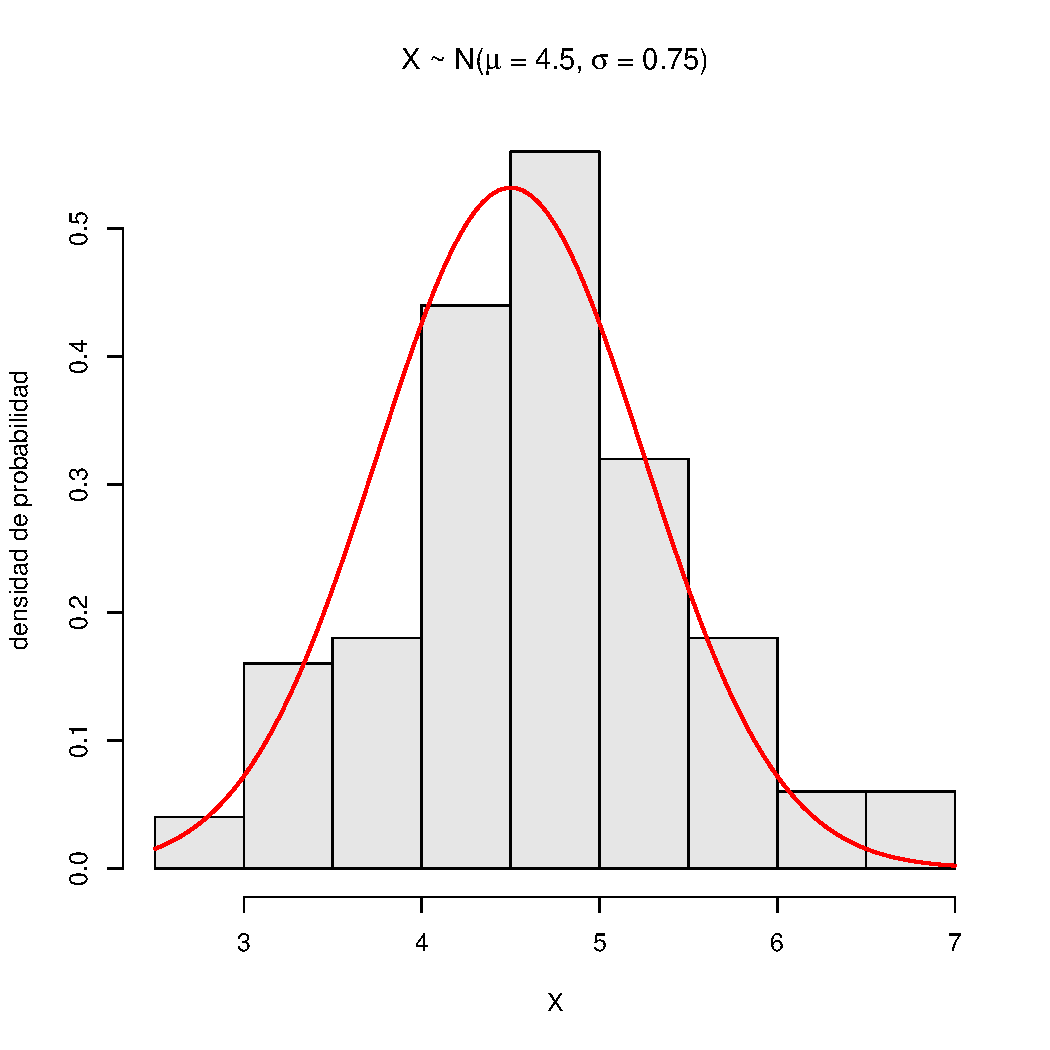
\includegraphics[width=\maxwidth]{figure/unnamed-chunk-6-1} 

\end{knitrout}

 Barras agrupadas 
\begin{knitrout}
\definecolor{shadecolor}{rgb}{0.969, 0.969, 0.969}\color{fgcolor}\begin{kframe}
\begin{alltt}
\hlkwd{barplot}\hlstd{(}\hlkwd{t}\hlstd{(tablaCont),} \hlkwc{main}\hlstd{=}\hlstr{"Gr?fico de barras (Estado, Ocupaci?n)"}\hlstd{,} \hlkwc{xlab}\hlstd{=}\hlstr{"Estado civil"}\hlstd{,}
\hlkwc{ylab}\hlstd{=}\hlstr{"Ocupaci?n"}\hlstd{,} \hlkwc{beside}\hlstd{=}\hlnum{TRUE}\hlstd{,} \hlkwc{legend.text}\hlstd{=}\hlnum{TRUE}\hlstd{)}
\end{alltt}
\end{kframe}
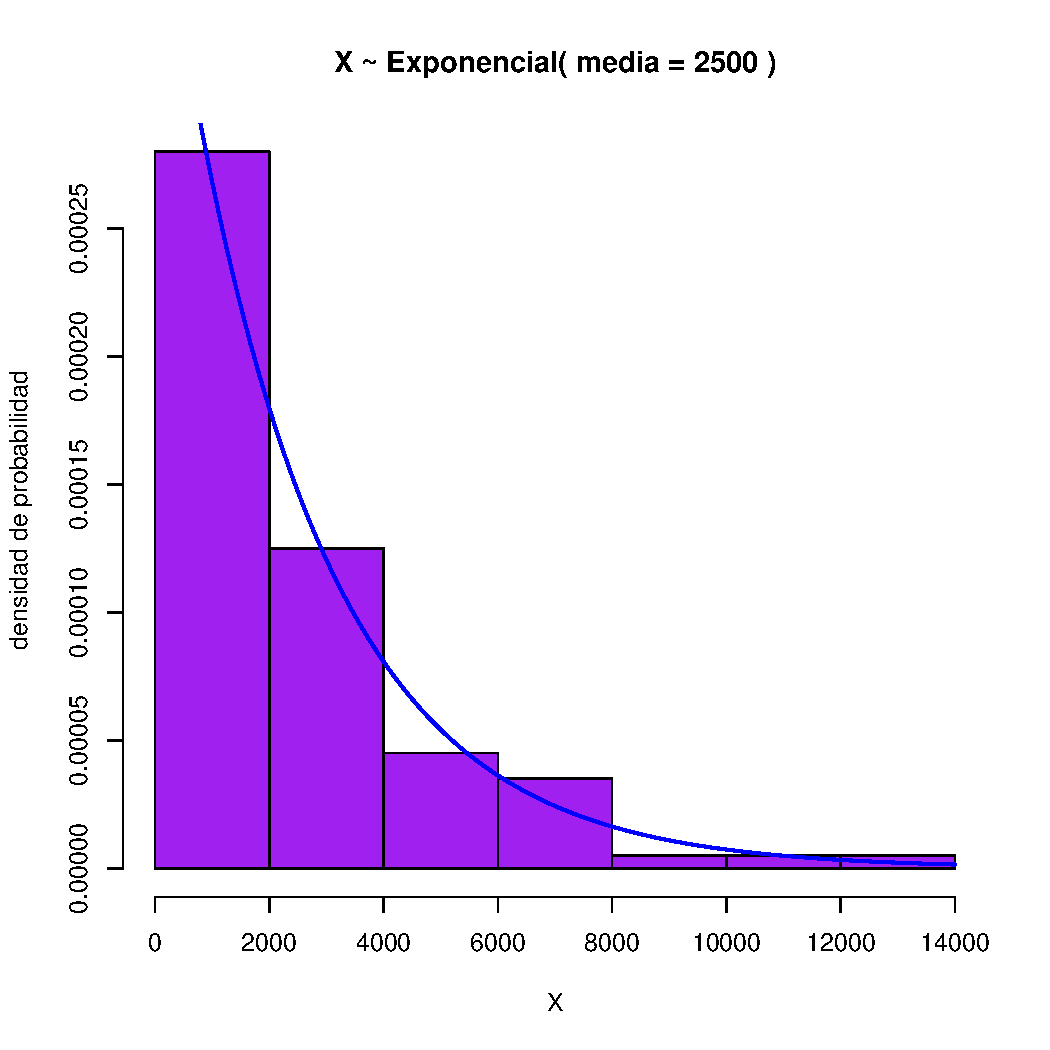
\includegraphics[width=\maxwidth]{figure/unnamed-chunk-7-1} 

\end{knitrout}

Al usar beside =FALSE se obtiene el mismo gr?fico de la instrucci?n anterior.
\begin{knitrout}
\definecolor{shadecolor}{rgb}{0.969, 0.969, 0.969}\color{fgcolor}\begin{kframe}
\begin{alltt}
\hlkwd{barplot}\hlstd{(tablaCont,} \hlkwc{main}\hlstd{=}\hlstr{"Gr?fico de barras (Ocupaci?n, Estado)"}\hlstd{,} \hlkwc{xlab}\hlstd{=}\hlstr{"Ocupaci?n\textbackslash{}n"}\hlstd{,}
\hlkwc{ylab}\hlstd{=}\hlstr{"Estado civil"}\hlstd{,} \hlkwc{beside}\hlstd{=}\hlnum{TRUE}\hlstd{,} \hlkwc{legend.text}\hlstd{=}\hlnum{TRUE}\hlstd{)}
\end{alltt}
\end{kframe}

\includegraphics[width=\maxwidth]{figure/unnamed-chunk-8-1} 

\end{knitrout}

Calcula tablas de proporciones o de probabilidades. 
\begin{knitrout}
\definecolor{shadecolor}{rgb}{0.969, 0.969, 0.969}\color{fgcolor}\begin{kframe}
\begin{alltt}
\hlstd{op} \hlkwb{<-} \hlkwd{options}\hlstd{()}
\hlkwd{options}\hlstd{(}\hlkwc{digits}\hlstd{=}\hlnum{3}\hlstd{)}
\hlkwd{options}\hlstd{(}\hlstr{'digits'}\hlstd{)}
\end{alltt}
\begin{verbatim}
## $digits
## [1] 3
\end{verbatim}
\end{kframe}
\end{knitrout}

 
\end{document}



